\section{Design d'interfaces de l'application}

Pour montrer les nouvelles fonctions définies et vérifier la possibilité d'en réaliser, j'ai mis en oeuvre un design d'interfaces de l'application qui comprend 3 parties principales: 

\subsection{Créer un projet}

Il y a deux façon de créer un projet :

\begin{figure}[H]
\centering
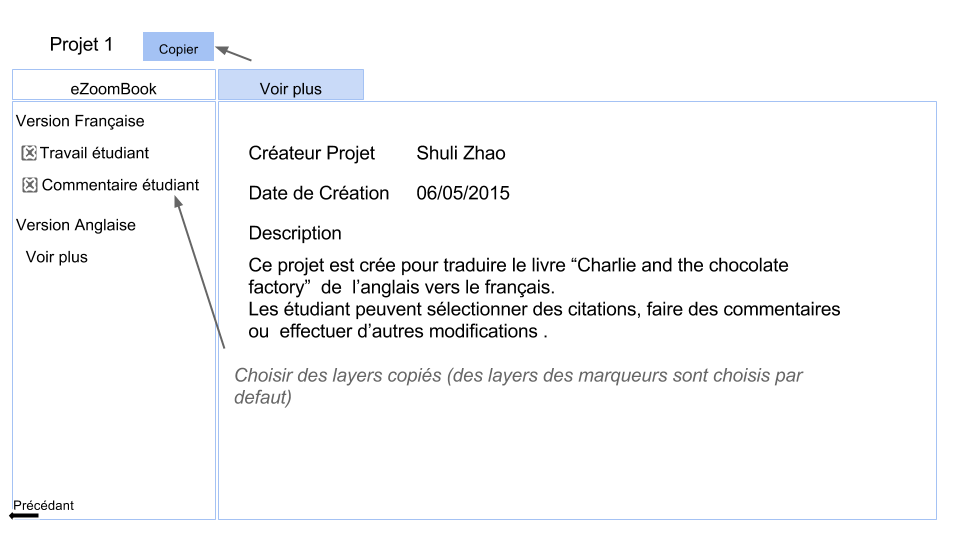
\includegraphics[width=\textwidth]{creer_projet}
\caption{Créer un projet à partir d'un projet existant}
\end{figure}

Quand on crée un projet à partir un projet existant, il faut choisir des layers publiques à copier. Des layers originals, des marqueurs et des séquences sont aussi conpiés automatiquement sans des informations d'éditeurs. 

\begin{figure}[H]
\centering
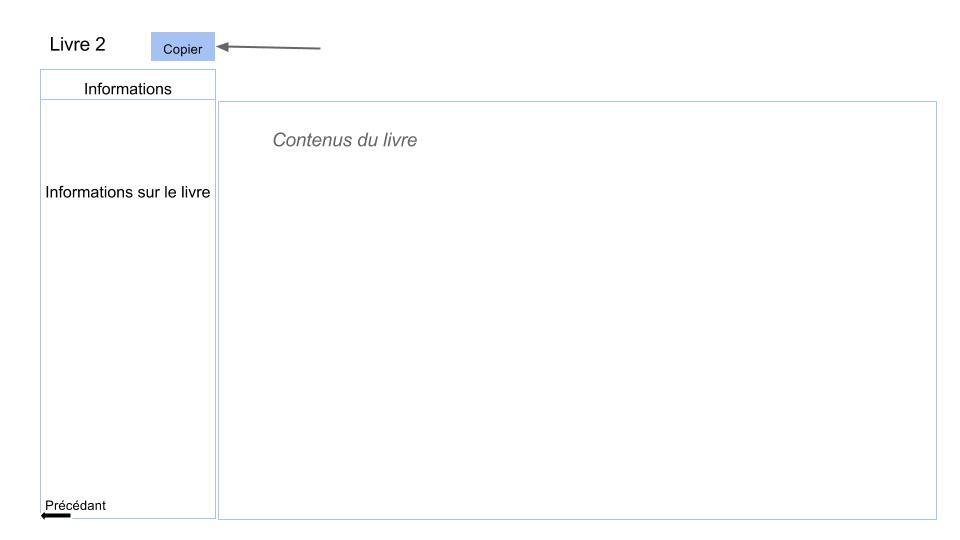
\includegraphics[width=\textwidth]{creer_livre}
\caption{Créer un projet à partir d'un livre}
\end{figure}

\begin{figure}[H]
\centering
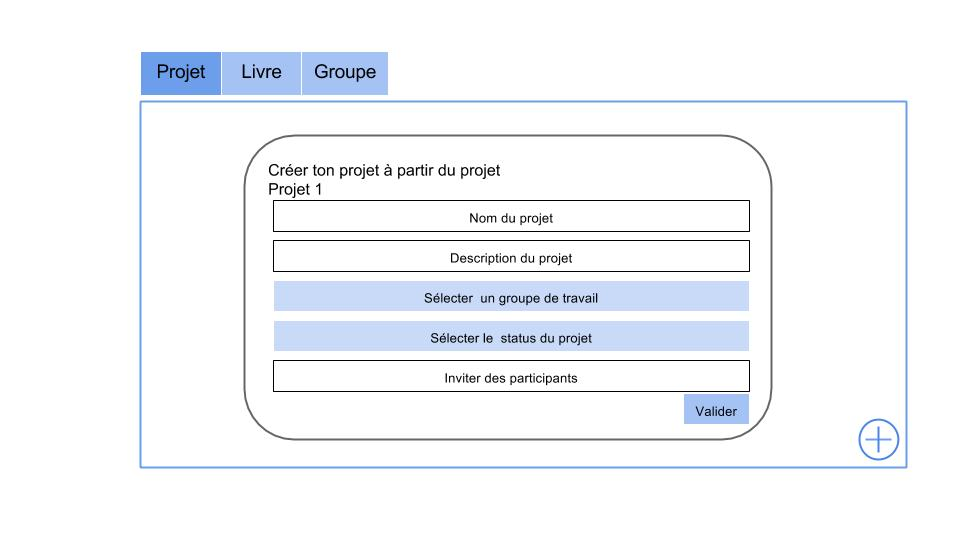
\includegraphics[width=\textwidth]{creer_info}
\caption{Remplir toutes les informations demandées}
\end{figure}

\subsection{Distribuer un projet}

Sur le page d'un layer original, à droite il y a toutes les finalités, quand on crée des séquences on sélecter des éditeurs dans la création, mais on peux aussi sélecter des éditeurs pour des autres finalités quand on entre dans l'édition de la finalité et clique le petit plus à côté.

\begin{figure}[H]
\centering
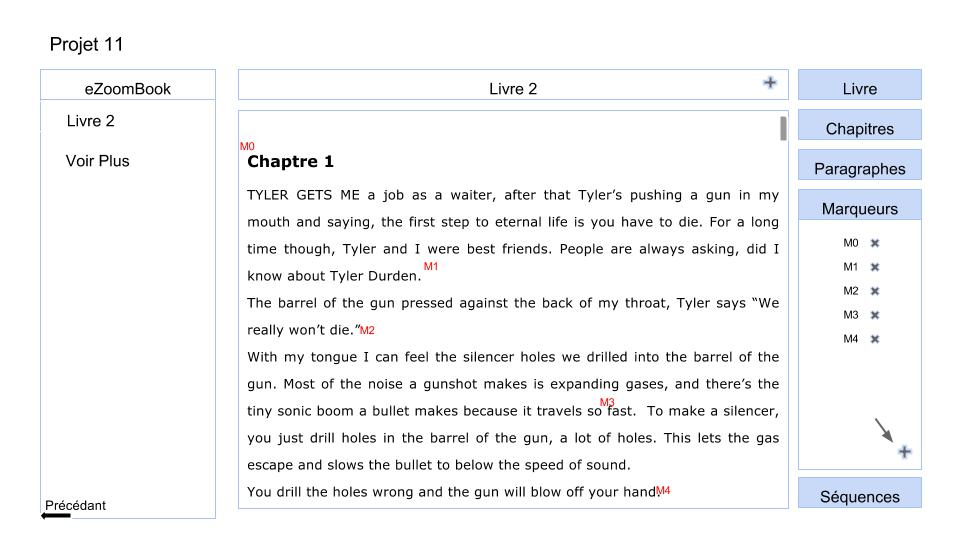
\includegraphics[width=\textwidth]{marqueurs}
\caption{Créer des marqueurs}
\end{figure}

\begin{figure}[H]
\centering
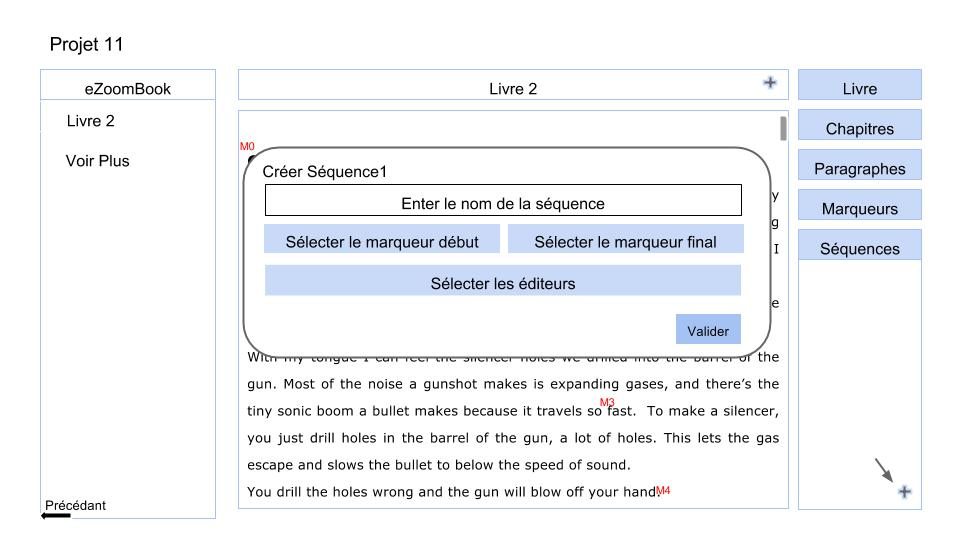
\includegraphics[width=\textwidth]{sequences}
\caption{Créer des séquences}
\end{figure}

\begin{figure}[H]
\centering
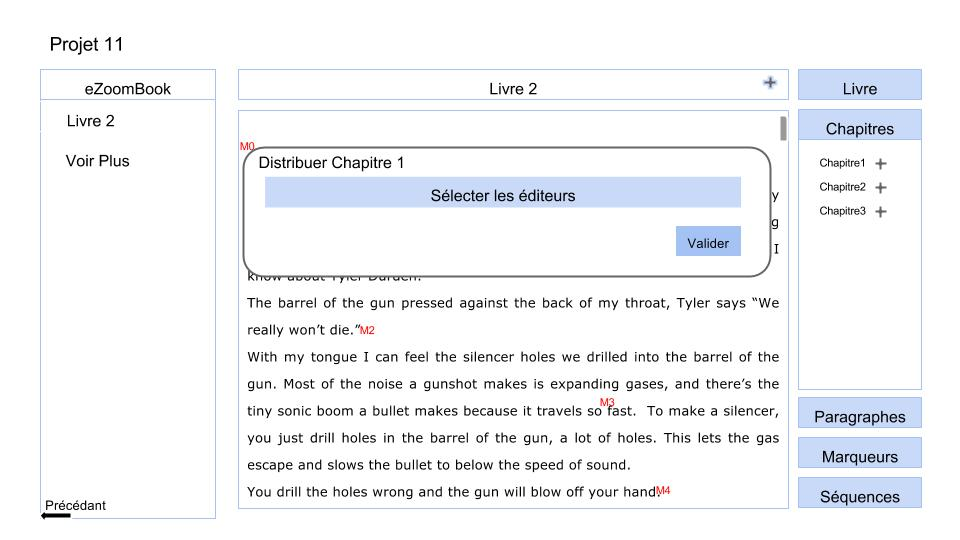
\includegraphics[width=\textwidth]{distribuer}
\caption{Distribuer des chapitres}
\end{figure}

\subsection{Contribuer dans un projet}

\subsubsection{Créer un layer}

Quand on crée un sous-layer d'un layer original, il faut choisir le type de finalité, mais si on crée un sous-layer d'un layer travail, il hérite la finalité de son parent layer.

\begin{figure}[H]
\centering
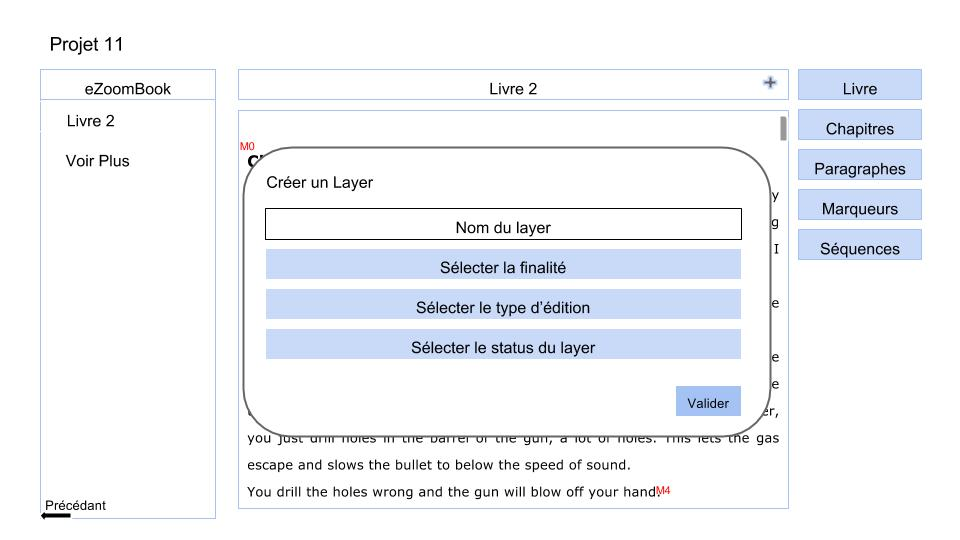
\includegraphics[width=\textwidth]{creer_layer}
\caption{Informations à remplir d'une création d'un sous-layer d'un layer original}
\end{figure}

\begin{figure}[H]
\centering
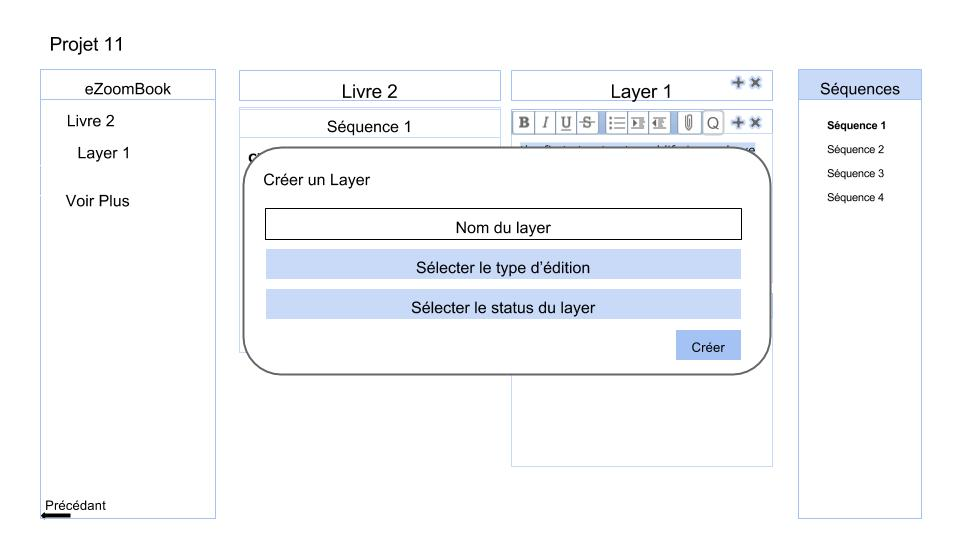
\includegraphics[width=\textwidth]{creer_commentaire}
\caption{Informations à remplir d'une création d'un sous-layer d'un layer travail}
\end{figure}

\subsubsection{Editer un layer}

Après la création, on va rentrer directement dans la contribution du layer. Sur le page, le layer à contribuer est mis à doite et son parent layer est à gauche qui permet d'un travail correspendant assez simple. Dans la édition d'un layer, on peut aussi sélecter tous les layers audessus en sélecter le nom du layer à gauche.

Dans des blocks permettant plusieurs types de manipulations, on peut faire des citation, écrire en multiformat et insérer des image, etc. C'est aussi possible d'insérer des parties nécessaires entres celles existantes en cliquent des petits plus et on vas avoir un parties audessous. Ca arrive aussi quand on veux une édition de certains parties d'un livre, il suffit de cliquer des petits croix de morceaux dispensables. Si on veux faire une citation, il faut juste cliquer sur le boutton Q et sélecter une partie de parent layer.

\begin{figure}[H]
\centering
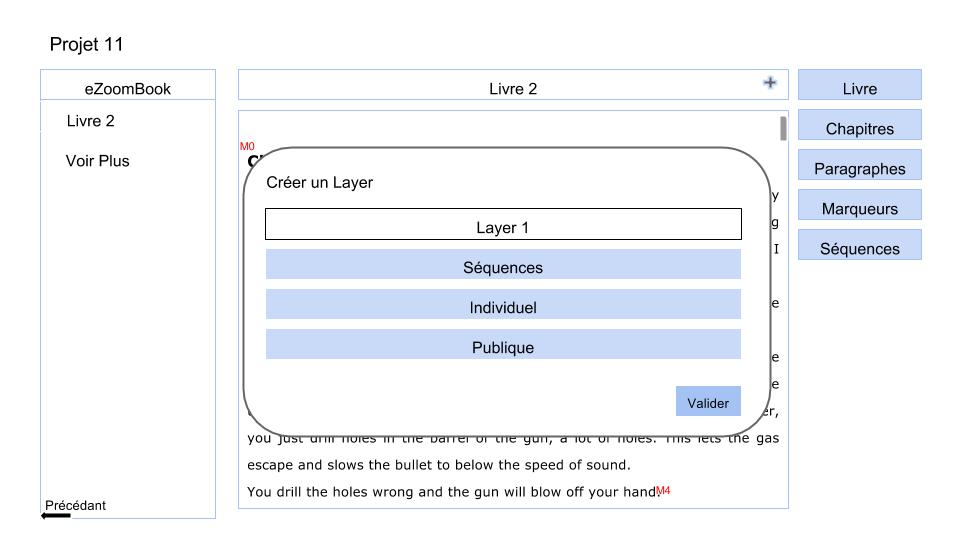
\includegraphics[width=\textwidth]{creer_indi}
\caption{Créer un layer individuel}
\end{figure}

\begin{figure}[H]
\centering
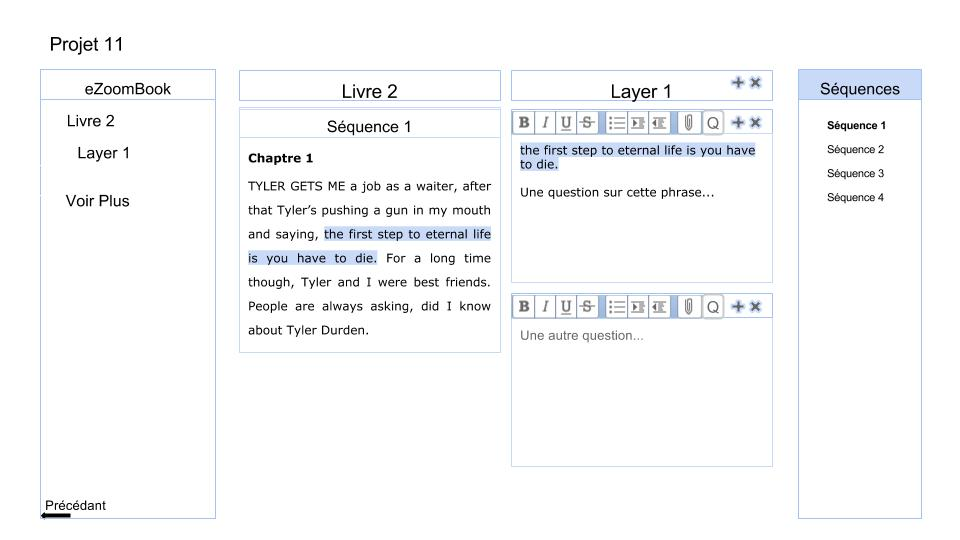
\includegraphics[width=\textwidth]{edition_indi}
\caption{Editer le layer individuel}
\end{figure}

\begin{figure}[H]
\centering
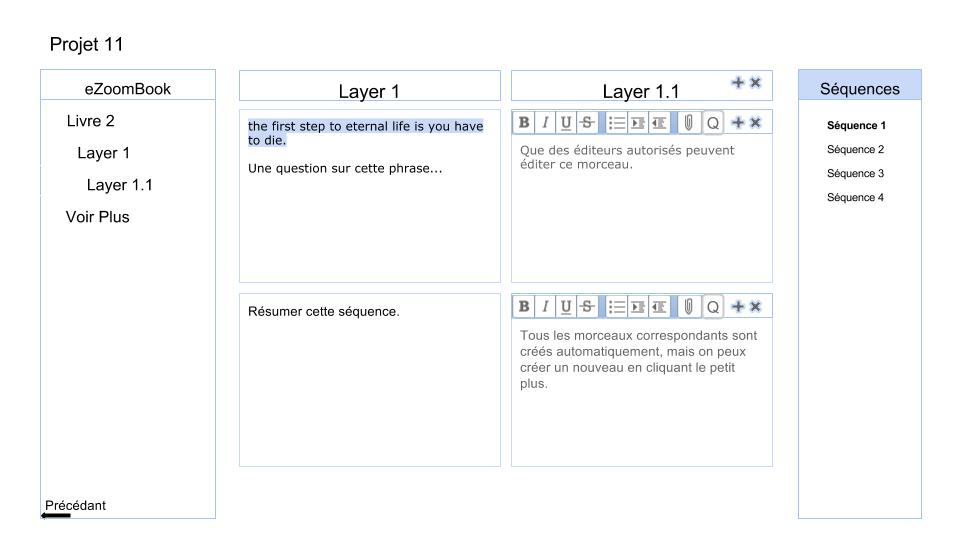
\includegraphics[width=\textwidth]{col_parent}
\caption{Un layer avec son parent layer}
\end{figure}

\begin{figure}[H]
\centering
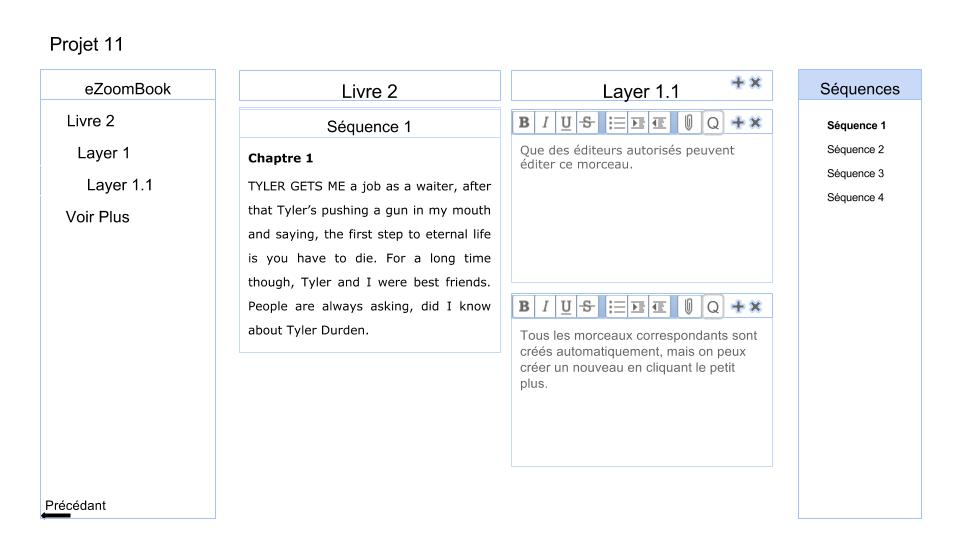
\includegraphics[width=\textwidth]{col}
\caption{Le layer avec son layer original}
\end{figure}